\documentclass[12pt,a4paper]{article}

% ---------------- BALÍKY ----------------
\usepackage[utf8]{inputenc}
\usepackage[slovak]{babel}
\usepackage[T1]{fontenc}
\usepackage{graphicx}
\usepackage{geometry}
\usepackage{amsmath}
\usepackage{amssymb}
\usepackage{float}
\usepackage{caption}
\usepackage{subcaption}
\usepackage{multirow}
\usepackage{booktabs} % Pre krajšie tabuľky (toprule, midrule...)

% Profesionálne formátovanie jednotiek a čísiel
\usepackage{siunitx}
\sisetup{
    output-decimal-marker = {,}, % Desatinná čiarka vo výstupe
    per-mode = symbol,
    group-digits = false, % Vypnutie medzier pre tisíce (voliteľné)
    exponent-product = \cdot
}

% ---------------- NASTAVENIA ----------------
\geometry{
    a4paper,
    total={170mm,257mm},
    left=20mm,
    top=20mm,
    bottom=20mm,
    right=20mm
}

\setlength{\parindent}{0pt}
\setlength{\parskip}{1em}

% Vlastné príkazy pre zjednodušenie zápisu
\newcommand{\R}[1]{R_{\mathrm{#1}}} % Napr. \R{ekv} spraví R_ekv (stojaté)

\begin{document}

% ---------------- TITULNÁ STRANA ----------------
\begin{titlepage}
    \begin{center}
        \Large \textsc{Vysoké učení technické v Brně}\\
        \vspace{0.5em}
        \huge \textsc{Fakulta informačních technologií}\\

        \vspace{2cm}

        % Logo
        
\includegraphics[width=0.5\linewidth]{files/logo_cz.png}

        \vspace{2cm}

        {\LARGE \textsc{Elektronika pro informační technologie}}\\
        \vspace{0.5em}
        {\Large 2025/2026}

        \vspace{3cm}

        {\Huge \textbf{Semestrální projekt}}\\

        \vfill
    \end{center}

    \begin{flushleft}
        \Large
        \textbf{Autor:} Michal Holeša (xholesm00)
    \end{flushleft}

    \vspace{0.5cm}

    \begin{flushleft}
        \Large
        Brno, 13.~12.~2025
    \end{flushleft}
\end{titlepage}

% ---------------- ÚLOHA 1 ----------------
\section*{Úloha 1: Metóda postupného zjednodušovania (Variant H)}

\subsection*{Zadané hodnoty}
Hodnoty sú prevzaté zo zadania pre skupinu H:

\begin{table}[h!]
    \centering
    \renewcommand{\arraystretch}{1.3}
    \begin{tabular}{|l|c|c|c|c|c|}
        \hline
        \textbf{Parameter} & $U_1$            & $U_2$           & $R_1$           & $R_2$           & $R_3$           \\ \hline
        \textbf{Hodnota}   & \qty{135}{\volt} & \qty{80}{\volt} & \qty{680}{\ohm} & \qty{600}{\ohm} & \qty{260}{\ohm} \\ \hline
        \hline
        \textbf{Parameter} & $R_4$            & $R_5$           & $R_6$           & $R_7$           & $R_8$           \\ \hline
        \textbf{Hodnota}   & \qty{310}{\ohm}  & \qty{575}{\ohm} & \qty{870}{\ohm} & \qty{355}{\ohm} & \qty{265}{\ohm} \\ \hline
    \end{tabular}
\end{table}

Celkové napätie: $U = U_1 + U_2 = 135 + 80 = \qty{215}{\volt}$.

\begin{figure}[H]
    \centering
    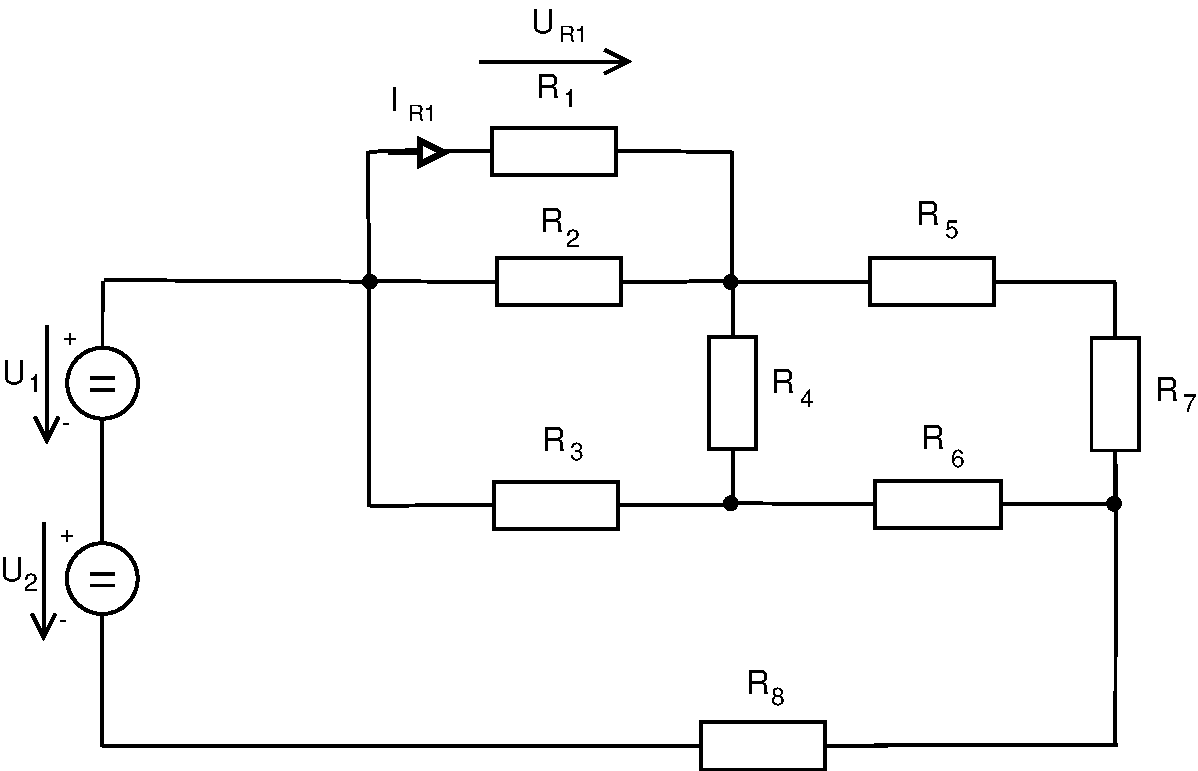
\includegraphics[width=0.5\linewidth]{files/obr/Pr1_2025.pdf}
    \caption*{Pôvodná schéma zapojenia}
\end{figure}

\subsection*{Postup výpočtu}

\textbf{1. Prvotné zjednodušenie odporov:}

Odpor $R_{12}$ (paralelná kombinácia $R_1, R_2$) a $R_{57}$ (sériová kombinácia $R_5, R_7$):
\begin{align*}
    R_{12} & = \frac{R_1 \cdot R_2}{R_1 + R_2} = \frac{680 \cdot 600}{680 + 600} = \qty{318.7500}{\ohm} \\
    R_{57} & = R_5 + R_7 = 575 + 355 = \qty{930.0000}{\ohm}
\end{align*}

\begin{figure}[H]
    \centering
    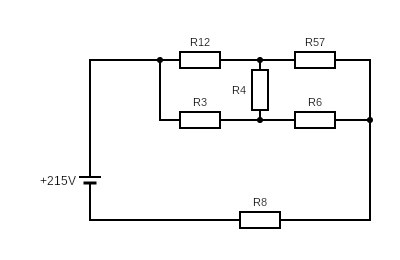
\includegraphics[width=0.4\linewidth]{files/1/circuit.png}
    \caption*{Schéma po prvotnom zjednodušení}
\end{figure}

\textbf{2. Transfigurácia trojuholník na hviezdu:}

Trojuholník tvorený odpormi $R_{57}, R_4, R_6$ nahradíme hviezdou $R_A, R_B, R_C$.
Súčet odporov v~trojuholníku: $\sum R_\Delta = R_{57} + R_4 + R_6 = \qty{2110}{\ohm}$.

\begin{align*}
    R_A & = \frac{R_{57} \cdot R_6}{\sum R_\Delta} = \frac{930 \cdot 870}{2110} \doteq \qty{383.4597}{\ohm} \\
    R_B & = \frac{R_{57} \cdot R_4}{\sum R_\Delta} = \frac{930 \cdot 310}{2110} \doteq \qty{136.6351}{\ohm} \\
    R_C & = \frac{R_6 \cdot R_4}{\sum R_\Delta} = \frac{870 \cdot 310}{2110} \doteq \qty{127.8199}{\ohm}
\end{align*}

\begin{figure}[H]
    \centering
    \begin{subfigure}[b]{0.45\textwidth}
        \centering
        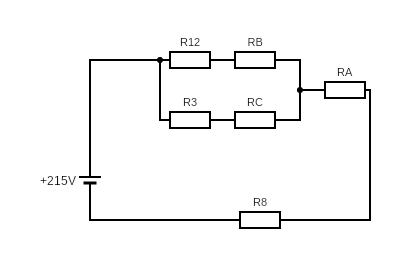
\includegraphics[width=0.9\linewidth]{files/1/circuit(1).png}
    \end{subfigure}
    \hfill
    \begin{subfigure}[b]{0.45\textwidth}
        \centering
        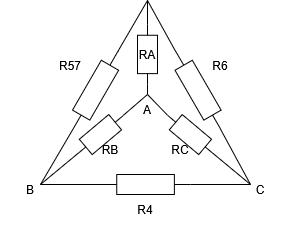
\includegraphics[width=0.7\linewidth]{files/1/hviezda.png}
    \end{subfigure}
    \caption*{Transfigurácia zapojenia (nahradenie trojuholníka hviezdou)}
\end{figure}

\textbf{3. Výpočet celkového odporu $\R{ekv}$:}

Obvod zjednodušíme na dve paralelné vetvy ($R_{12B}$ a~$R_{3C}$) v~sérii s~$R_8$ a~$R_A$.

\begin{align*}
    R_{12B} & = R_{12} + R_B = 318.7500 + 136.6351 = \qty{455.3851}{\ohm} \\
    R_{3C}  & = R_3 + R_C = 260 + 127.8199 = \qty{387.8199}{\ohm}
\end{align*}

Ekvivalentný odpor paralelnej časti $\R{p}$:
\begin{equation*}
    \R{p} = \frac{R_{12B} \cdot R_{3C}}{R_{12B} + R_{3C}} = \frac{455.3851 \cdot 387.8199}{455.3851 + 387.8199} \doteq \qty{209.4470}{\ohm}
\end{equation*}

Celkový odpor obvodu:
\begin{equation*}
    \R{ekv} = R_8 + R_A + \R{p} = 265 + 383.4597 + 209.4470 \doteq \qty{857.9067}{\ohm}
\end{equation*}

\begin{figure}[H]
    \centering
    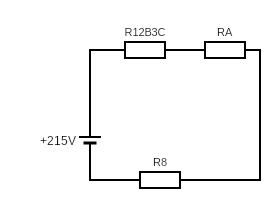
\includegraphics[width=0.3\linewidth]{files/1/circuit(2).png} \qquad
    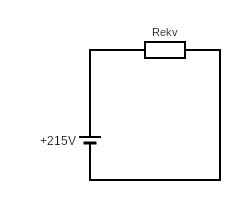
\includegraphics[width=0.3\linewidth]{files/1/circuit(3).png}
    \caption*{Finálne zjednodušenie obvodu na $\R{ekv}$}
\end{figure}

\textbf{4. Výpočet celkového prúdu a~spätný dopočet:}

\begin{align*}
    I                                                    & = \frac{U}{\R{ekv}} = \frac{215}{857.9067} \doteq \qty{0.2506}{\ampere}                  \\[1em]
    \text{Napätie na paralelnej časti } U_{\mathrm{p}}:  &                                                                                          \\
    U_{\mathrm{p}}                                       & = \R{p} \cdot I = 209.4470 \cdot 0.2506 \doteq \qty{52.4897}{\volt}                      \\[1em]
    \text{Prúd vetvou s~odporom } R_1 \; (I_{12B}):      &                                                                                          \\
    I_{12B}                                              & = \frac{U_{\mathrm{p}}}{R_{12B}} = \frac{52.4897}{455.3851} \doteq \qty{0.1153}{\ampere} \\[1em]
    \text{Napätie na odpore } R_1 \; (U_{R1} = U_{R12}): &                                                                                          \\
    U_{R1}                                               & = R_{12} \cdot I_{12B} = 318.7500 \cdot 0.1153 \doteq \mathbf{\qty{36.7519}{\volt}}      \\[1em]
    \text{Výsledný prúd odporom } R_1:                   &                                                                                          \\
    I_{R1}                                               & = \frac{U_{R1}}{R_1} = \frac{36.7519}{680} \doteq \mathbf{\qty{0.0541}{\ampere}}
\end{align*}

\newpage

% ---------------- ÚLOHA 2 ----------------
\section*{Úloha 2: Théveninova veta (Variant G)}

\subsection*{Zadané hodnoty}
Hodnoty sú prevzaté zo zadania pre skupinu G:

\begin{table}[h!]
    \centering
    \renewcommand{\arraystretch}{1.3}
    \begin{tabular}{|c|c|c|c|c|c|c|}
        \hline
        $U_1$            & $R_1$           & $R_2$           & $R_3$           & $R_4$           & $R_5$           & $R_6$           \\ \hline
        \qty{180}{\volt} & \qty{315}{\ohm} & \qty{615}{\ohm} & \qty{180}{\ohm} & \qty{460}{\ohm} & \qty{120}{\ohm} & \qty{250}{\ohm} \\ \hline
    \end{tabular}
\end{table}

\begin{figure}[H]
    \centering
    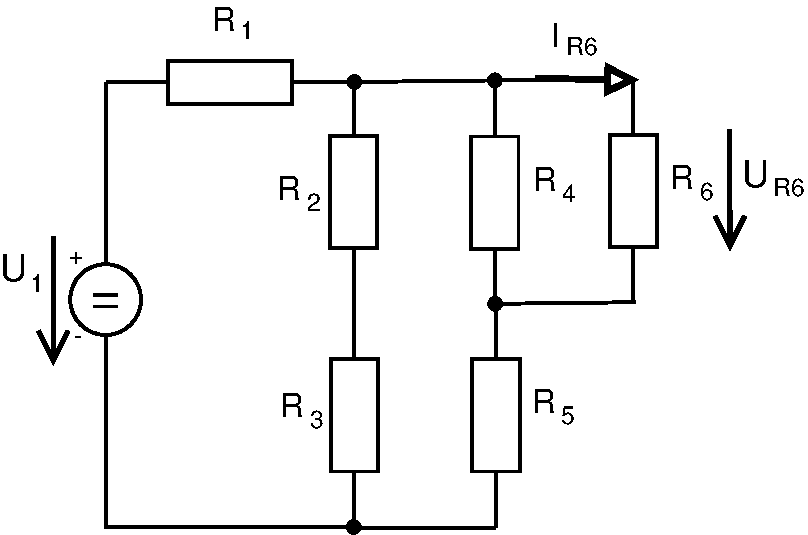
\includegraphics[width=0.5\linewidth]{files/obr/Pr2_2025.pdf}
    \caption*{Schéma zapojenia pre Úlohu 2}
\end{figure}

\subsection*{1. Výpočet napätia naprázdno ($U_i$)}
Najskôr stanovíme napätie na svorkách rezistora $R_4$ pri odpojenej záťaži $R_6$. Obvod zjednodušíme postupným zlučovaním odporov.

\begin{figure}[H]
    \centering
    
\includegraphics[width=0.23\linewidth]{files/2/UI/circuit.png} \hfill
    
\includegraphics[width=0.23\linewidth]{files/2/UI/circuit(1).png} \hfill
    
\includegraphics[width=0.23\linewidth]{files/2/UI/circuit(2).png} \hfill
    
\includegraphics[width=0.23\linewidth]{files/2/UI/circuit(3).png}
    \caption*{Postupné zjednodušovanie obvodu pre výpočet $U_i$}
\end{figure}

\begin{align*}
    R_{23}   & = R_2 + R_3 = 615 + 180 = \qty{795}{\ohm}                                                                  \\
    R_{45}   & = R_4 + R_5 = 460 + 120 = \qty{580}{\ohm}                                                                  \\
    R_{2345} & = \frac{R_{23} \cdot R_{45}}{R_{23} + R_{45}} = \frac{795 \cdot 580}{795 + 580} \doteq \qty{335.345}{\ohm} \\
    \R{ekv}  & = R_1 + R_{2345} = 315 + 335.345 = \qty{650.345}{\ohm}
\end{align*}

Ďalej vypočítame celkový prúd zo zdroja a~rozloženie napätia:

\begin{align*}
    I_{G}     & = \frac{U_1}{\R{ekv}} = \frac{180}{650.345} \doteq \qty{0.2768}{\ampere} \\
    U_{R1}    & = R_1 \cdot I_{G} = 315 \cdot 0.2768 \doteq \qty{87.192}{\volt}          \\
    U_{R2345} & = U_1 - U_{R1} = 180 - 87.192 = \qty{92.808}{\volt}
\end{align*}

Pretože $U_{R45} = U_{R2345}$, môžeme určiť prúd tečúci vetvou s~rezistorom $R_4$:

\begin{align*}
    I_{R4} & = I_{R45} = \frac{U_{R45}}{R_{45}} = \frac{92.808}{580} = \qty{0.16}{\ampere} \\
    U_i    & = U_{R4} = R_4 \cdot I_{R4} = 460 \cdot 0.16 = \qty{73.6}{\volt}
\end{align*}

\subsection*{2. Výpočet Théveninovho odporu ($R_i$)}
Pre výpočet vnútorného odporu nahradíme zdroj napätia skratom a~vyjadríme odpor videný zo svoriek rezistora $R_6$ (t.~j. paralelne k~$R_4$).

\begin{align*}
    R_{123}  & = \frac{R_1 \cdot R_{23}}{R_1 + R_{23}} = \frac{315 \cdot 795}{315 + 795} \doteq \qty{225.608}{\ohm}             \\
    R_{1235} & = R_{123} + R_5 = 225.608 + 120 = \qty{345.608}{\ohm}                                                            \\
    R_i      & = \frac{R_{1235} \cdot R_4}{R_{1235} + R_4} = \frac{345.608 \cdot 460}{345.608 + 460} \doteq \qty{197.343}{\ohm}
\end{align*}

\begin{figure}[H]
    \centering
    
\includegraphics[width=0.23\linewidth]{files/2/RI/circuit.png} \hfill
    
\includegraphics[width=0.23\linewidth]{files/2/RI/circuit(1).png} \hfill
    
\includegraphics[width=0.23\linewidth]{files/2/RI/circuit(2).png} \hfill
    
\includegraphics[width=0.23\linewidth]{files/2/RI/circuit(3).png}
    \caption*{Postup zjednodušovania obvodu pre výpočet vnútorného odporu $R_i$}
\end{figure}

\subsection*{3. Výpočet prúdu a~napätia na $R_6$}
Použijeme náhradný Théveninov obvod pripojený k~záťaži $R_6$:

\begin{align*}
    I_{R6} & = \frac{U_i}{R_i + R_6} = \frac{73.6}{197.343 + 250} \doteq \qty{0.1645}{\ampere} \\
    U_{R6} & = R_6 \cdot I_{R6} = 250 \cdot 0.1645 \doteq \mathbf{\qty{41.125}{\volt}}
\end{align*}

\begin{figure}[H]
    \centering
    
\includegraphics[width=0.3\linewidth]{files/2/circuit.png}
    \caption*{Náhradný Théveninov obvod so záťažou $R_6$}
\end{figure}

\newpage

% ---------------- PREHĽAD VÝSLEDKOV ----------------
\section*{Prehľad výsledkov} % Opravené z "Přehled výsledků"

\begin{table}[h!]
    \centering
    \renewcommand{\arraystretch}{1.5}
    \setlength{\tabcolsep}{12pt}
    \begin{tabular}{|c|c|l|}
        \hline
        \textbf{Úloha}     & \textbf{Variant}       & \textbf{Výsledky}                \\ \hline % Opravené z "Varianta"
        \multirow{2}{*}{1} & \multirow{2}{*}{H}     & $U_{R1} = \qty{36.7519}{\volt}$  \\
                           &                        & $I_{R1} = \qty{0.0541}{\ampere}$ \\ \hline
        \multirow{2}{*}{2} & \multirow{2}{*}{G}     & $U_{R6} = \qty{41.1250}{\volt}$  \\
                           &                        & $I_{R6} = \qty{0.1645}{\ampere}$ \\ \hline
        \multirow{2}{*}{3} & \multirow{2}{*}{\dots} & $U_{R4} = \dots \, \si{\volt}$   \\
                           &                        & $I_{R4} = \dots \, \si{\ampere}$ \\ \hline
        \multirow{2}{*}{4} & \multirow{2}{*}{\dots} & $|U_{L2}| = \dots \, \si{\volt}$ \\
                           &                        & $\varphi_{L2} = \dots ^\circ$    \\ \hline
        5                  & \dots                  & $u_c(t) = \dots$                 \\ \hline
    \end{tabular}
    \caption*{Súhrnná tabuľka výsledkov}
\end{table}

\end{document}